%!TEX root = ../Thesis.tex
\chapter{Uiteenzetting Vooronderzoek}
\label{ch:onderzoek}
\lhead{\emph{Uiteenzetting Vooronderzoek}}

In dit hoofdstuk wordt antwoord gegeven op de volgende vragen door middel van de onderzoeksmethoden beschreven in~\ref{subsec:onderzoeksmethoden}

\begin{itemize}
\item Wat is de huidige kennis van computerlogica onder de werknemers van DPI?
\item Is er extra training nodig om met de ontwikkelomgeving aan de slag te gaan?
\item Welke componenten zullen gemaakt moeten worden?
	\begin{itemize}
	\item Wat zijn de huidige taken van een programmeur bij het maken van een virtuele omgeving?
	\item Welke tools bestaan er al?
	\item Wat zijn de juiste abstracties van de componenten? 
	\end{itemize}
\item Is het mogelijk de componenten cross-platform te maken?
	\begin{itemize}
	\item Welke platformen zijn relevant?
	\item Wat zijn de verschillende mogelijkheden van deze platforms?
	\end{itemize}
\end{itemize}

\section{Wat is de huidige kennis van computerlogica onder de werknemers van DPI?}
Om een idee te krijgen van de huidige kennis van de niet-programmeurs is er begonnen met een enquête over programmeur terminologie \ref{appendix:oreintatieintervieuw:enquete} en een interview over vorige werk ervaringen. \ref{appendix:oreintatieintervieuw:interview}. 

De enquête schept een goed beeld over hoe groot de vorige programmeur-ervaring van de niet-programmeurs is. De correcte terminologie begrijpen van een onderwerp toont namelijk aan dat de er naast het in aanraking met het onderwerp ook bewust kennis is gezocht of gedeeld. En het interview geeft context aan de enquête.

\subsection{Conclusie}
Uit de enquête en het interview blijkt dat er nauwelijks kennis is van programmeren. Wel is er ervaring met 3D software wat het werken in het begin met \gls{ue4} makkelijker zal maken en er sneller gefocust kan worden op het logica aspect.

\section{Is er extra training nodig om met de ontwikkelomgeving aan de slag te gaan?}
Omdat er geen kennis is over het Blueprint systeem van \gls{ue4} of eerder contact is geweest met programmeren, is er besloten om een aantal workshops te geven waarin de niet-programmeurs de basis van Blueprints leren.

\subsection{Conclusie}
In de workshop \ref{appendix:workshop1} is er een introductie gemaakt in de \gls{ue4} en Blueprints. Omdat de niet-programmeurs van een 3D modelling achtergrond komen zijn de verschillen in best practises tussen een game engine en 3d software benadrukt.

In de workshop \ref{appendix:workshop2} krijgen de niet-programmeurs uitleg over Blueprints en de VRInteractions plugin en maken zij zelfstandig een opdracht.

In de workshop \ref{appendix:workshop3} wordt er een complexe opdracht gemaakt en wordt er verwacht dat de niet-programmeurs zelfstandig problemen kunnen oplossen.

\section{Welke componenten zullen gemaakt moeten worden?}
\label{sec:welkeComponenten}
De ontwikkelde componenten zijn gebaseerd op de problemen die de niet-programmeurs tegen komen tijdens het maken en opzetten van \gls{vr} omgevingen. DPI heeft eerder een volledige \gls{vr} ervaring gemaakt in Unity maar deze was niet interactief en gaf weinig input voor het kiezen van componenten. 

Tijdens het schrijven van de scriptie zijn de volgende \gls{vr} omgevingen gemaakt met de VRInteractions plugin

\begin{itemize}
	\item Een fly-trough door een menselijk lichaam
	\item Een appartement waarvan o.a. het meubilair en de vloer dynamisch aangepast kon worden
	\item Een demo van een machine uit een fabriek
	\item Een virtuele omgeving van een tentoonstelling
	\item Een leeromgeving rond het colosseum
	\item Een demo omgeving van de VRInteractions plugin
\end{itemize}

Op basis van de functionaliteit en problemen van deze projecten is de VRInteractions plugin ontwikkeld.

\subsection{Wat zijn de huidige taken van een programmeur in het maken van een Virtuele omgeving?}
DPI focust zich voornamelijk op het maken van exposities in \gls{vr}. Een voorbeeld van een use-case is een opstelling op een beurs vervangen door een \gls{vr} omgeving.

Om de omgeving in te stellen, te starten of tussen omgevingen te navigeren wordt een menu gebruikt waarin de gebruiker opties kan kiezen. Daarnaast wordt er tijdens de demo zelf interactie gebruikt om op een engaging manier informatie te tonen. 

De taken van een programmeur komen in de meeste exposities neer op:

\begin{itemize}
	\item Opzetten van het project
	\item Programmeren van menu en transitie van levels
	\item Programmeren van de triggers voor animaties 
\end{itemize}


\subsection{Welke tools bestaan er al?}
Op het moment van schrijven zijn er een aantal \gls{vr} interactieve producties gemaakt in \gls{ue4}. De producties die het meest lijken op de expositie projecten van DPI zijn:
 
\begin{itemize}
	\item The Rose and I~\footnote{http://store.steampowered.com/app/396060/}
	\item Henry~\footnote{https://storystudio.oculus.com/en-us/henry/}
	\item The Body VR~\footnote{https://www2.oculus.com/experiences/rift/967071646715932/}
\end{itemize}

Deze producties gebruiken voornamelijk het kijken naar elementen als interactie vorm. Maar geen van de projecten heeft bekend gemaakt een toolkit te gebruiken of gesproken over hun implementatie van de interactie.

\subsection{Wat zijn de juiste abstracties van de componenten?}
Blueprints maakt het mogelijk om bepaalde opties te groeperen en als geavanceerd te labelen. 

\begin{figure}[H]
  \centering
    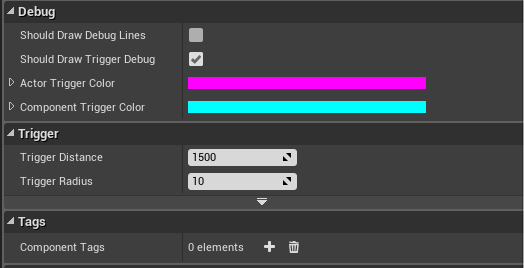
\includegraphics[width=\linewidth/2,height=\textheight/2,keepaspectratio]{Onderzoek_VoorbeeldGeavanceerdDicht}
    \caption{Voorbeeld van de geavanceerde opties die verborgen zijn.}
  \label{fig:advOptiesHidden}    
\end{figure}

\begin{figure}[H]
  \centering
    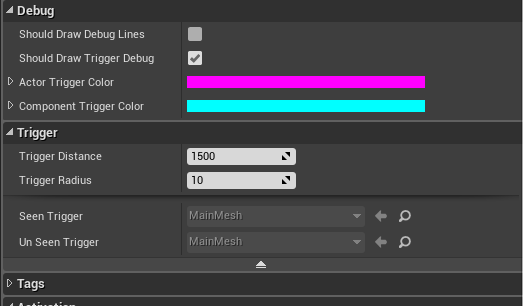
\includegraphics[width=\linewidth/2,height=\textheight/2,keepaspectratio]{Onderzoek_VoorbeeldGeavanceerdOpen}
    \caption{Voorbeeld van de geavanceerde opties die zichtbaar zijn.}
  \label{fig:advOptiesVisible}
\end{figure}

Dit zorgt ervoor dat de componenten zo abstract mogelijk gecodeerd kunnen worden en de opties die voor onduidelijkheid zorgen verborgen kunnen worden. Ook is het mogelijk om versimpelde versies van functies te maken die aanspreekbaar zijn in Blueprints.

\subsection{Conclusie}
Op basis van de gemaakte projecten en de workshops zijn de volgende componenten ontwikkeld voor de VRInteractions plugin:

\begin{itemize}
	\item Een game mode voor een demo waarin de speler kan rondlopen en een voor een fly-through demo
	\item Een speler klasse per game mode
	\item Een component wat verantwoordelijk is voor de input van de speler
	\item Een component wat verantwoordelijk is voor de camera van de speler
	\item Een component die events afvuurt als er naar een object gekeken word
	\item Een HUD die het mogelijk maakt op basis de look events informatie te tonen
	\item Een 3D menu die zijn opties in een cirkel toont
	\item Een object wat verplaats kon worden door middel van ernaar te kijken.
\end{itemize}

Deze zijn in code zo abstract mogelijk opgezet en vervolgens door groepering van de instellingen en het toevoegen van hulp functies versimpelt in Blueprints.

\section{Is het mogelijk de componenten cross-platform te maken?}
De huidige componenten zijn geschreven met het kijken naar objecten als interactie vorm, een interactie vorm die op elk VR device mogelijk is. 

Voor de GearVR, Vive, en de Oculus kan er gebruik gemaakt worden van de camera positie van de speler. Voor \gls{vr} brillen zoals de Cardboard word de positie van de camera niet automatisch gecorrigeerd en moet de headtracking zelf geïmplementeerd worden. 

Voor elke bril die de camera van de speler automatisch update werken de componenten out of the box.

\subsection{Welke platforms zijn relevant?}
\label{subsec:platforms}
De huidige \gls{vr} headsets die in productie zijn, dus niet in een beta fase, zijn de GearVR, Oculus, Vive en de Cardboard. De Oculus en Vive zijn geschikt voor uitgebreide producties van hoge kwaliteit maar de GearVR is gelimiteerd aan de grafische kracht van de gebruikte mobiel, maar werken alleen op een telefoon uit de Samsung Galaxy serie. 

De Cardboard is ook gelimiteerd aan de kracht van de mobiel die gebruikt word maar kan met Android telefoon gebruikt worden. Dit limiteert de grafische mogelijkheden zover dat er geen comfortabele framerate en responsiveness bereikt kan worden.

\subsection{Wat zijn de verschillende mogelijkheden van deze platforms?}
Omdat de controllers van de GearVR, Oculus en de Vive hardware matig van elkaar verschillen is het erg lastig om deze alle drie te ondersteunen. 

De GearVR maakt namelijk gebruik van een touchpad op de bril of een aangesloten gamepad. De Oculus en Vive hebben beiden eigen controllers ontwikkeld maar deze bevatten verschillende knoppen en door het hardware matige verschil moet hier dubbele code voor geschreven worden.

\subsection{conclusie}
Door de interactie te beperken tot het kijken naar objecten is het mogelijk voor de plugin om alle huidige headsets in productie te ondersteunen op de Cardboard gebaseerde headsets na.

Voor dit onderzoek ondersteunen wij daarom alle brillen op de Cardboard na. De GearVR voor de lage instap kosten voor consumenten en portabiliteit en de Oculus en Vive voor hun hogere grafische mogelijkheden.